%!TEX program = xelatex
%!TEX TS-program = xelatex
%!TEX encoding = UTF-8 Unicode

\documentclass[a4paper, 12pt, centering]{article}

\input{config}

\title{\yihao{基于神经渲染的三维场景重建与传统图形渲染流程对比}}
\author{\xiaoerhao{杨皓然}\footnote{电子邮件: 2330142@bjtu.edu.cn，学号: 23301142}\\[2ex]
\sanhao 北京交通大学软件学院\\[2ex]
}
\date{\sanhao\today}
\begin{document}

\begin{center}

\includegraphics[width=0.4\textwidth]{images/BJTU_emblem.png}
\end{center}
\vspace{1.2cm}

\begingroup
\let\newpage\relax% Void the actions of \newpage
\maketitle
\endgroup
\newpage

\begin{abstract}
神经渲染将可微优化、神经场表示与传统图形学中的相机投影、可见性和体渲染模型结合起来，为三维场景重建与新视角合成提供了新的技术路线。本文围绕静态场景的多视角图像输入，比较传统显式重建与渲染流程、NeRF 类神经辐射场流程以及以 3D Gaussian Splatting 为代表的高效神经渲染流程。传统流程依赖 SfM/MVS、网格重建、纹理映射和显式材质光照设置，具有较好的几何可解释性与编辑性；神经渲染流程则通过图像监督优化连续或半显式的场景表示，在训练视角附近的新视角合成质量和自动化程度上具有优势。本文从表示形式、渲染过程、质量评价、控制能力和流程效率五个方面设计对比框架，并讨论神经渲染在稀疏视角、相机位姿误差、视角外推、几何编辑和光照材质分离方面可能引入的新问题。研究目标不是比较单张图像的生成效果，而是分析神经渲染如何改变三维图形学管线中“重建表示”和“渲染输出”的分工。
\end{abstract}

\begin{keys}
神经渲染；神经辐射场；新视角合成；三维重建；3D Gaussian Splatting（3DGS）
\end{keys}

\begin{enabstract}
Neural rendering combines differentiable optimization and neural field representations with camera projection, visibility, and volume rendering models from computer graphics. This paper studies 3D scene reconstruction and novel view synthesis from multi-view images, and compares three pipelines: traditional explicit reconstruction and rendering, NeRF-style neural radiance fields, and efficient neural rendering represented by 3D Gaussian Splatting. The traditional pipeline relies on SfM/MVS, mesh reconstruction, texture mapping, and explicit material or lighting configuration, which provides interpretable geometry and direct editing interfaces. Neural rendering optimizes continuous or semi-explicit scene representations from image supervision, and often improves visual fidelity and automation near the training views. We design a comparison framework in terms of representation, rendering process, quality, controllability, and efficiency, and discuss new limitations such as sparse-view instability, pose errors, view extrapolation artifacts, weak geometric editability, and entangled material-lighting effects.
\end{enabstract}

\begin{enkeys}
neural rendering; neural radiance fields; novel view synthesis; 3D reconstruction; 3D Gaussian Splatting
\end{enkeys}
\newpage

\tableofcontents
\newpage

\section{引言}
传统计算机图形学通常从显式场景描述出发生成图像。一个典型流程包括几何建模、材质与纹理制作、光照设置、相机配置以及光栅化或路径追踪渲染。对于真实场景，如果希望从照片恢复可渲染模型，则还需要通过运动恢复结构（Structure from Motion, SfM）估计相机位姿，通过多视图立体（Multi-View Stereo, MVS）获得点云或网格，再进行纹理映射、网格清理和渲染参数调整。该流程的优势在于结构清晰：几何、材质、光照和相机是相对独立的对象，因而便于检查、修改和导入传统渲染引擎；其不足也同样明显，即真实场景的反光、半透明、细薄结构、遮挡边界和纹理缺失会显著增加重建与修复成本。

神经渲染的出现改变了上述流程中“显式建模优先”的假设。Tewari 等人的综述将神经渲染概括为结合经典图形学与生成式机器学习的图像或视频合成方法，并强调其核心在于对相机、姿态、几何、外观和语义结构等场景属性提供显式或隐式控制\cite{tewari2020state}。这一定义表明，神经渲染并不是脱离图形学的二维图像生成，而是在投影、可见性、体渲染、反射外观等图形学约束下引入可学习表示。Xie 等人的 neural fields 综述进一步指出，坐标网络可以把空间或时空中的物理量参数化为连续场，从而统一描述形状、外观、密度、辐射度等多种视觉计算对象\cite{xie2022neuralfields}。

在这一背景下，NeRF 将静态场景表示为从三维位置和观察方向到体密度、颜色的连续函数，并通过沿相机射线的体渲染积分合成图像\cite{mildenhall2020nerf}。这一模型把多视角图像监督、神经网络表示和经典体渲染方程连接起来，成为神经渲染领域的代表性方法。此后，Instant-NGP、Plenoxels、TensoRF、Mip-NeRF、3D Gaussian Splatting 等工作分别从编码结构、显式体素、张量分解、反走样和实时 splatting 角度改进训练速度、渲染速度和视觉质量\cite{muller2022instant,yu2022plenoxels,chen2022tensorf,barron2021mipnerf,kerbl2023gaussians}。

本文选择“基于神经渲染的三维场景重建与传统图形渲染流程对比”作为研究主题，原因在于该问题能够直接落到图形学过程本身：输入是多视角图像，输出是可从新视角渲染的三维场景表示。这里的“有无大模型”不再指文本大模型是否参与语义规划，而是指传统显式图形管线与引入神经场、可微渲染或可优化高斯表示后的渲染管线之间的差异。本文关注四个问题：第一，神经渲染是否提升新视角合成质量；第二，场景控制性是否因隐式或半显式表示而发生变化；第三，从图像到可渲染结果的流程效率是否提高；第四，神经渲染是否引入新的不稳定性，例如几何不一致、视角外推失败、光照材质耦合和编辑困难。

本文的主要工作是构建一个统一的三维重建与新视角渲染比较框架。该框架把传统 SfM/MVS/mesh/texture 渲染流程、NeRF 类神经辐射场流程和 3D Gaussian Splatting（3DGS）高效神经渲染流程放在相同输入、相同测试视角和相同评价指标下讨论。通过这种设计，论文比较的不是某一张图像是否“更好看”，而是不同图形学管线在场景表示、渲染机制、可控编辑、效率和局限上的系统差异。

\section{相关技术现状}
\subsection{传统摄影测量与显式渲染流程}
传统图形学管线以显式场景表示为中心。对于人工创建的虚拟场景，艺术家或程序首先构建网格、曲面或体数据，再为对象指定纹理、材质、法线、光源和相机；渲染器根据几何可见性、着色模型和光照传输计算最终图像。对于真实场景重建，常见工具链通常由 COLMAP 完成 SfM 与相机位姿估计\cite{schonberger2016sfm,schonberger2016mvs}，再由 OpenMVS、Meshroom/AliceVision 或 Blender 摄影测量相关插件完成深度估计、点云融合、网格化、纹理贴图和资产整理。该路线的核心优势是可解释性：网格顶点、三角面片、纹理图和光源参数都具有明确语义，因此可以被传统建模软件和游戏引擎直接编辑。

显式流程的主要困难来自重建误差与外观建模的不完备。多视图重建依赖跨视角特征匹配和局部光度一致性，弱纹理表面、镜面反射、透明物体、细小结构和动态干扰都会破坏匹配稳定性。即使得到网格，纹理映射仍可能出现错位、接缝和模糊；如果希望在新光照下重新渲染，还需要进一步分离几何、反照率、粗糙度和光照。Tewari 等人在综述中指出，传统逼真图形学已经能从手工构建的场景表示合成高质量图像，但自动获得形状、材质、光照等场景属性仍然是重要瓶颈\cite{tewari2020state}。这正是神经渲染希望介入的位置。

\subsection{神经渲染与神经场表示}
神经渲染并不是单一算法，而是一类将可学习模型嵌入图形学图像形成过程的方法。按照 Tewari 等人的归纳，神经渲染的关键问题包括控制变量如何提供、管线中哪些部分被学习、控制是显式还是隐式、结果是确定性还是随机性，以及模型能否泛化到新场景\cite{tewari2020state}。这些维度与传统图形学关心的几何、相机、材质、光照和动画并不矛盾，而是把其中部分环节改写为数据驱动优化问题。

神经场为这类方法提供了统一表示。Xie 等人将 neural fields 定义为用坐标网络参数化空间或时空中物理量的函数表示\cite{xie2022neuralfields}。在图形学任务中，这些物理量可以是有符号距离、密度、颜色、辐射度、形变或人体姿态相关的属性。Scene Representation Networks 早期展示了连续神经场作为三维结构感知场景表示的可能性\cite{sitzmann2019srn}；DeepSDF 则用连续有符号距离函数表示三维形状，说明隐式神经表示可以提供不同于三角网格的几何建模方式\cite{park2019deepsdf}。这些工作共同构成了 NeRF 及后续神经渲染方法的表示基础。

\subsection{NeRF、加速结构与方法演进}
NeRF 的贡献在于把连续神经场与经典体渲染方程结合起来。给定空间位置 $\mathbf{x}$ 和观察方向 $\mathbf{d}$，网络输出体密度 $\sigma$ 和颜色 $\mathbf{c}$，再沿相机射线积分得到像素颜色\cite{mildenhall2020nerf}。与直接生成二维图像不同，NeRF 的输出受三维坐标、视线方向、透射率和可见性的约束，因此能够在训练视角附近合成连续变化的新视角。

原始 NeRF 的主要代价来自逐像素、逐采样点的网络查询。若图像分辨率为 $H\times W$，每条射线采样 $N_s$ 个点，单次 MLP 前向计算代价记为 $C_{\mathrm{MLP}}$，则单帧渲染的主导复杂度可近似写为 $O(HW N_s C_{\mathrm{MLP}})$。因此，后续工作大体沿两条路线展开：一是改善采样和抗锯齿，例如 Fourier Features、Mip-NeRF、Mip-NeRF 360 和 Zip-NeRF 分别从高频编码、锥台积分、无界场景参数化和网格抗锯齿角度提高质量\cite{tancik2020fourier,barron2021mipnerf,barron2022mipnerf360,barron2023zipnerf}；二是把昂贵的连续网络查询转移到更显式的存储结构中，例如 PlenOctrees、SNeRG、Plenoxels、TensoRF 和 Instant-NGP 分别通过烘焙、稀疏体素、张量分解和多分辨率哈希编码降低训练或渲染开销\cite{yu2021plenoctrees,hedman2021snerg,yu2022plenoxels,chen2022tensorf,muller2022instant}。

\begin{figure}[htbp]
\centering
\begin{tabular}{c|c|c|c|c}
\hline
显式几何 & 连续辐射场 & 加速辐射场 & 半显式高斯 & 可编辑/可重光照高斯 \\
\hline
SfM/MVS/mesh & NeRF & Instant-NGP/TensoRF & 3DGS & SuGaR/GaussianShader/2DGS \\
\hline
拓扑清晰 & 体渲染一致 & 查询更快 & 实时 splatting & 几何或外观约束增强 \\
\hline
\end{tabular}
\caption{从显式重建到神经渲染的技术演进关系}
\label{fig:evolution}
\end{figure}

\subsection{3DGS 及其近年扩展}
3D Gaussian Splatting 是近年高效神经渲染的重要代表。它从 SfM 点云初始化三维高斯，用可微优化更新高斯的位置、协方差、透明度和视角相关颜色，再通过排序和 splatting 进行实时渲染\cite{kerbl2023gaussians}。与 NeRF 的逐射线采样不同，3DGS 先把三维高斯投影到屏幕空间，再在 tile 内排序和 alpha 合成；若某像素受到 $K$ 个有效 splat 影响，则像素合成代价可近似看作 $O(K)$，主导开销转移为高斯投影、tile 分配、局部排序和显存访问。该设计减少了大量 MLP 查询，且更符合 GPU 光栅化式并行访问模式，因此通常具有更高的交互渲染速度。

3DGS 的效率来自半显式表示，但它的弱点也来自这一表示。三维高斯是离散体元而不是拓扑表面，优化后可能形成漂浮高斯、过大高斯或多视角不一致的局部结构。近两年的工作主要围绕这些问题展开：GaussianShader 在三维高斯上引入简化着色函数和法线估计，以改善反射表面重建\cite{jiang2023gaussianshader}；GaussianEditor 利用三维高斯的局部可选择性支持文本指令驱动的局部编辑\cite{wang2023gaussianeditor}；SuGaR 通过表面对齐正则和 Poisson 重建从高斯中提取可编辑网格\cite{guedon2023sugar}；2D Gaussian Splatting 将三维体高斯压缩为面向表面的二维高斯盘，以增强多视角几何一致性\cite{huang2024twodgs}。这些扩展说明，3DGS 不是“NeRF 的终点”，而是把神经渲染问题重新推向几何、材质、编辑和物理一致性约束。

\subsection{几何控制与真实场景鲁棒性}
高质量新视角图像并不自动意味着高质量几何。为获得更明确的表面，NeuS 和 VolSDF 将神经隐式表面与体渲染联系起来，尝试从多视角图像中恢复更稳定的 SDF 表面\cite{wang2021neus,yariv2021volsdf}。这类方法说明，图像合成质量和几何可编辑性是相关但不同的目标，实验中需要分别讨论。

真实输入还会带来相机位姿误差、光照变化、临时遮挡和稀疏视角等问题。BARF 将相机位姿与 NeRF 表示联合优化，用于缓解位姿不准对重建的影响\cite{lin2021barf}。NeRF in the Wild 面向互联网照片集合，引入外观编码和瞬态分量处理光照变化与临时遮挡\cite{martinbrualla2021nerfw}。RegNeRF 则关注少量输入视角下的正则化问题，说明神经渲染在数据不足时容易产生退化解\cite{niemeyer2022regnerf}。这些研究为本文的结果讨论提供了边界：神经渲染提升了自动化和视觉质量，但其稳定性依赖视角覆盖、相机质量、场景静态性和训练约束。

\section{方法设计}
\subsection{总体对比框架}
本文将实验对象抽象为同一个输入输出问题：给定同一静态场景的多视角图像 $\{I_i\}$ 及其相机参数 $\{K_i,R_i,t_i\}$，构建一个可以从新相机视角 $v$ 渲染图像 $\hat{I}_v$ 的场景表示。传统流程、NeRF 流程和 3DGS 流程的差异不在最终是否能输出图像，而在于中间场景表示和渲染方式不同。

为了保证比较公平，三条管线使用相同的图像集合、训练/测试划分和测试相机路径。评价时同时记录图像质量、耗时、资源消耗和编辑能力。图像质量可用 PSNR、SSIM、LPIPS 等指标衡量，其中 PSNR 和 SSIM 用于衡量像素误差与结构相似性，LPIPS 用于补充感知相似性；效率包括从输入图像到可渲染表示的总时间、单帧渲染时间和模型或资产大小；控制能力则从几何编辑、材质光照分离、相机路径外推和传统引擎兼容性几个方面进行定性比较。

\begin{figure}[htbp]
\centering
\begin{tabular}{c|c|c|c}
\hline
流程 & 输入 & 中间表示 & 输出 \\
\hline
传统显式流程 & 多视角图像与相机 & SfM 点云、MVS 网格、纹理、材质 & 光栅化或路径追踪图像 \\
NeRF 类流程 & 多视角图像与相机 & 连续密度与颜色场 & 体渲染新视角图像 \\
3DGS 流程 & 多视角图像与相机 & 可优化三维高斯集合 & splatting 新视角图像 \\
\hline
\end{tabular}
\caption{三类三维重建与渲染流程的数据流差异}
\label{fig:pipeline}
\end{figure}

\subsection{传统显式重建与渲染管线}
传统管线由四个阶段组成。第一阶段是相机估计和稀疏重建，使用 SfM 从多视角图像中匹配特征点并估计相机内外参，得到稀疏点云。第二阶段是稠密重建和网格生成，通过 MVS、深度融合或表面重建获得三角网格。第三阶段是资产整理，包括网格简化、孔洞修复、法线调整和纹理映射。第四阶段是在 Blender 或同类渲染器中设置相机路径、材质和光照，输出测试视角图像。

该管线的场景表示可以写成
\[
S_{\mathrm{mesh}}=\{V,F,T,M,L\},
\]
其中 $V$ 表示顶点，$F$ 表示面片，$T$ 表示纹理，$M$ 表示材质参数，$L$ 表示光照设置。渲染过程由传统渲染器完成，优势是每个变量都有明确含义，可单独修改；缺点是重建失败会直接表现为网格破洞、纹理拉伸或接缝，且反光、透明和弱纹理区域很难通过简单 MVS 得到可靠几何。

\subsection{NeRF 类神经辐射场管线}
NeRF 管线使用相同图像和相机参数，但不显式生成三角网格。它学习一个函数
\[
F_\Theta:(\mathbf{x},\mathbf{d})\rightarrow(\sigma,\mathbf{c}),
\]
其中 $\mathbf{x}$ 为空间位置，$\mathbf{d}$ 为观察方向，$\sigma$ 为体密度，$\mathbf{c}$ 为颜色。对一条相机射线 $\mathbf{r}(t)=\mathbf{o}+t\mathbf{d}$，像素颜色由体渲染积分近似得到：
\[
\hat{C}(\mathbf{r})=\sum_{j} T_j\left(1-\exp(-\sigma_j\delta_j)\right)\mathbf{c}_j,
\]
其中 $T_j$ 表示射线到第 $j$ 个采样点前的累积透射率，$\delta_j$ 为相邻采样点距离。训练目标是最小化渲染颜色与真实训练图像像素之间的误差。

该管线的关键变化是：场景表示从可直接编辑的网格和纹理，变为由参数 $\Theta$ 控制的连续辐射场。其优点是能够通过图像监督吸收复杂外观和视角相关效果，减少显式网格清理；缺点是训练和渲染成本较高，且几何、材质、光照往往纠缠在同一表示中。若需要提取网格，通常还要额外执行密度阈值化、marching cubes 或 SDF 转换，这些步骤会带来新的误差。

\subsection{高效神经渲染管线}
高效神经渲染管线用于观察神经渲染在效率维度上的改进。若采用 Instant-NGP，场景仍可看作辐射场，但坐标输入先经过多分辨率哈希编码，再由小型 MLP 输出密度和颜色，从而减少网络容量与训练时间\cite{muller2022instant}。若采用 3D Gaussian Splatting，场景表示为一组三维高斯：
\[
S_{\mathrm{3DGS}}=\{(\mu_k,\Sigma_k,\alpha_k,\mathbf{h}_k)\}_{k=1}^{N},
\]
其中 $\mu_k$ 是高斯中心，$\Sigma_k$ 是协方差，$\alpha_k$ 是透明度，$\mathbf{h}_k$ 表示球谐颜色系数。渲染时将三维高斯投影到屏幕空间，并按深度进行 alpha 合成。

与 NeRF 相比，3DGS 减少了沿每条射线大量采样和 MLP 查询的开销，因此更适合实时浏览和交互式展示。与传统 mesh 相比，它又不是拓扑明确的表面模型，难以像编辑三角网格一样直接修改边、面、UV 和材质。因此，本文把 3DGS 作为神经渲染效率改进的代表，而不是把它视为传统显式建模的简单替代。

\subsection{实验变量与比较维度}
本文后续实验将围绕三组变量展开。第一组是方法变量，包括传统 mesh+texture 渲染、NeRF 类辐射场和 3DGS。第二组是输入变量，包括完整多视角输入、稀疏视角输入和较大视角外推。第三组是流程变量，包括人工清理程度、训练或优化时间、参数调节次数和渲染速度。

比较结论将从四个问题展开。第一，结果质量是否提升：观察测试视角图像的误差指标和视觉细节。第二，控制性是否变化：比较能否单独编辑几何、材质、光照和相机。第三，效率是否提高：比较建模、训练、优化和渲染时间。第四，是否产生新局限：记录漂浮物、模糊、几何不一致、显存占用、外推失败和材质光照不可分离等现象。通过这些维度，本文能够把神经渲染的优势和代价同时放入计算机图形学管线中讨论。

\subsection{理论复杂度与管线差异}
三类方法的计算代价来源并不相同。传统 mesh 管线在重建阶段需要进行特征匹配、深度估计和表面重建，渲染阶段则主要依赖可见三角面片的光栅化或路径追踪。NeRF 类方法把显式表面替换为连续体场，单帧渲染需要对每个像素沿射线采样并查询网络，因此推理代价与像素数、采样数和网络前向计算量同时相关。3DGS 则把计算集中到高斯投影、tile 内排序和 alpha 合成，避免了大量逐采样点 MLP 查询，但需要保存和访问大量高斯参数。

\begin{table}[htbp]
\centering
\caption{三类流程的表示、渲染代价与主要瓶颈}
\label{tab:pipeline-complexity}
\begin{tabular}{p{0.22\textwidth}p{0.25\textwidth}p{0.25\textwidth}p{0.18\textwidth}}
\hline
流程 & 场景表示 & 渲染主导代价 & 主要瓶颈 \\
\hline
传统显式流程 & 点云、网格、纹理、材质 & 可见几何光栅化或路径追踪；与可见面片、光照采样有关 & 重建和纹理清理成本高 \\
NeRF 类流程 & 连续密度与颜色场 & 约为 $O(HW N_s C_{\mathrm{MLP}})$ & 采样和 MLP 查询密集 \\
3DGS 流程 & 可优化三维高斯集合 & 高斯投影、tile 排序和每像素 $O(K)$ alpha 合成 & 显存访问、排序和漂浮高斯 \\
\hline
\end{tabular}
\end{table}

\section{实验与对比}
\subsection{实验设置}
实验采用 NeRF Synthetic 数据集中的 \texttt{lego} 场景作为受控合成场景。该场景结构稳定、轮廓清晰、背景干净，适合在已知相机与透明背景条件下比较不同重建表示的基本差异。实验使用训练视角构建场景表示，并在 20 个测试视角上导出 RGB 图像进行评价。由于该场景不能覆盖真实采集噪声、复杂材质和开放背景，真实场景验证与多场景验证分别标记为 \texttt{TODO\_3} 和 \texttt{TODO\_4}。

本文比较三种流程。传统显式流程采用基于轮廓约束的 visual hull 基线：利用训练视角 RGBA 图像中的 alpha mask 对三维体素网格进行雕刻，得到显式点云/体素外壳；随后将该显式几何投影回训练图像采样颜色，并在测试视角下通过 z-buffer point splatting 渲染。该方法不使用神经网络，也不进行可微优化，因此可作为依赖显式几何和传统投影关系的基线。NeRF 类方法采用 Nerfstudio 中的 \texttt{nerfacto}，3DGS 类方法采用 \texttt{splatfacto}。二者均训练 30000 次迭代，并在相同测试相机上导出图像。完整硬件、软件版本与训练超参数仍需统一记录，见 \texttt{TODO\_5}。

评价指标包括 PSNR、SSIM、最差视角指标和指标标准差。PSNR 反映像素级误差，SSIM 反映局部结构相似性，标准差和最差视角用于观察跨视角稳定性。LPIPS 可补充感知相似性，但当前结果尚未完成该指标计算，因此表中以 \texttt{TODO\_1} 标记。Nerfstudio 方法的单帧渲染时间也需要在同一硬件和同一 \texttt{ns-render dataset} 方式下实测，本文暂不填入推断值，见 \texttt{TODO\_2}。

\subsection{定量结果}
\begin{table}[htbp]
\centering
\caption{Lego 场景 20 个测试视角上的定量结果}
\label{tab:metrics}
\begin{tabular}{lccccc}
\hline
方法 & PSNR $\uparrow$ & 最差 PSNR & SSIM $\uparrow$ & 最差 SSIM & LPIPS $\downarrow$ \\
\hline
Visual Hull & $15.62\pm0.33$ & 15.06 & $0.701\pm0.014$ & 0.685 & \texttt{TODO\_1} \\
Nerfacto & $21.13\pm2.07$ & 17.91 & $0.873\pm0.032$ & 0.815 & \texttt{TODO\_1} \\
Splatfacto & $28.28\pm4.25$ & 23.41 & $0.955\pm0.018$ & 0.923 & \texttt{TODO\_1} \\
\hline
\end{tabular}
\end{table}

表 \ref{tab:metrics} 表明，Visual Hull 的平均 PSNR 为 15.62，SSIM 为 0.701，明显低于两种神经渲染方法。Nerfacto 的平均 PSNR 和 SSIM 分别提升到 21.13 和 0.873，说明体密度、颜色和可见性的联合优化能够比轮廓外壳更好地解释测试视角图像。Splatfacto 取得最高的 28.28 PSNR 和 0.955 SSIM，说明三维高斯表示在该合成场景中能够更精确地逼近测试视角像素分布。与此同时，Splatfacto 的 PSNR 标准差也最大，说明其平均质量最高但跨视角收益并不完全均匀，仍需结合失败视角和更多场景判断稳定性。

\subsection{定性对比与误差分析}
\begin{figure}[htbp]
\centering
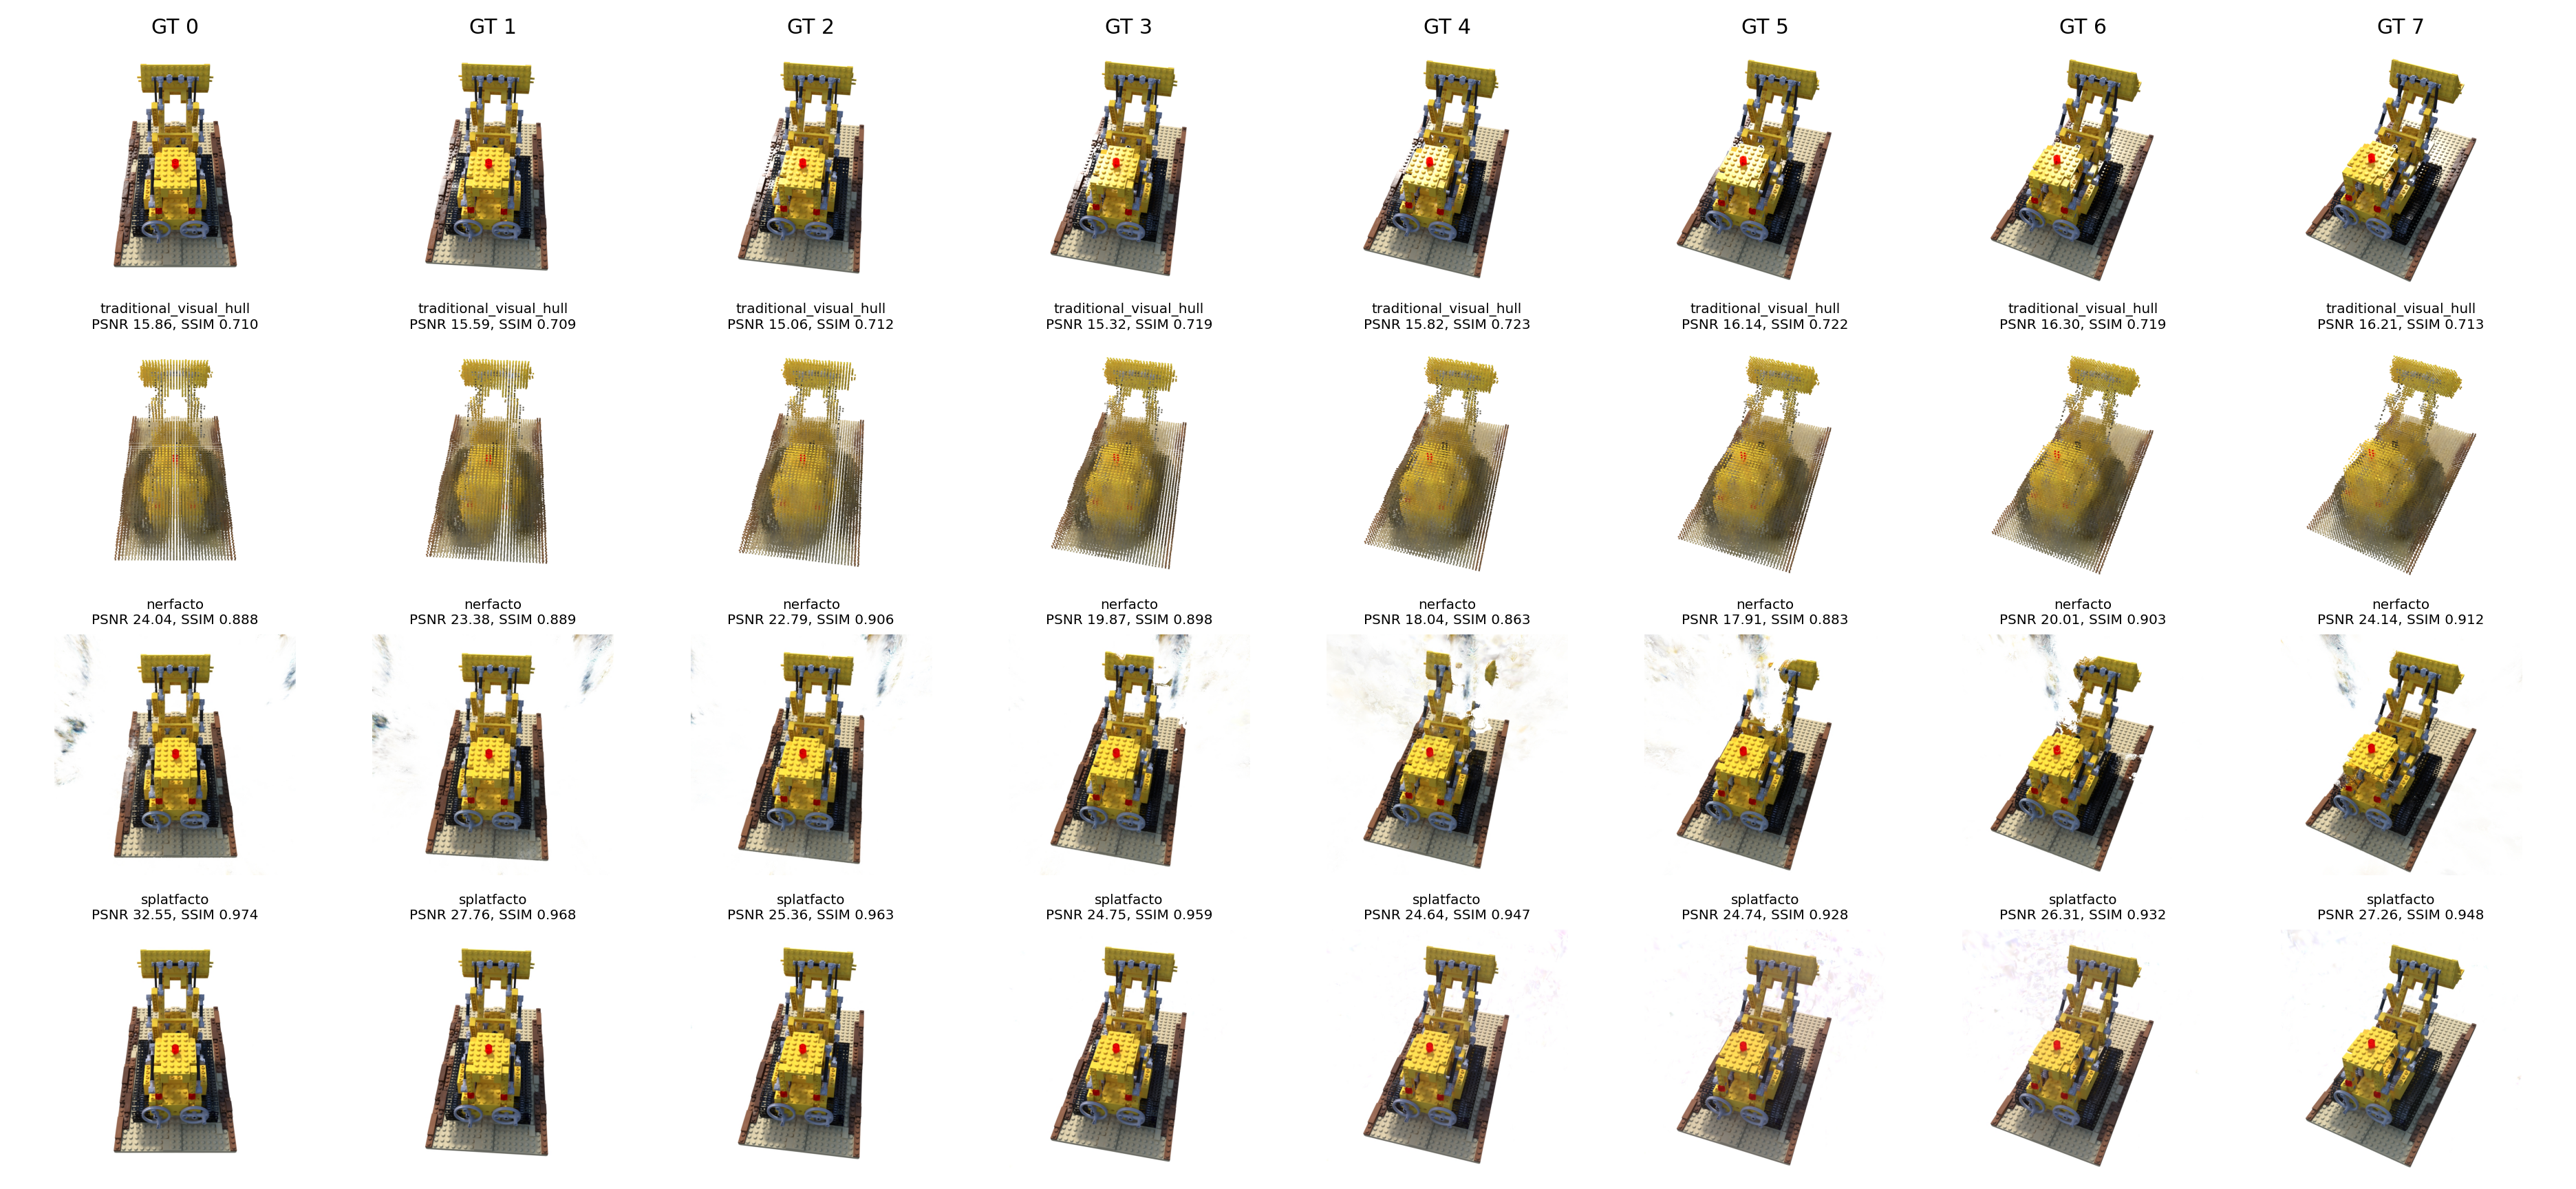
\includegraphics[width=0.95\textwidth]{images/experiments/lego_comparison.png}
\caption{Lego 测试视角的定性对比。每一列对应同一测试视角；各行依次为真实图像、Visual Hull、Nerfacto 和 Splatfacto。}
\label{fig:comparison}
\end{figure}

\begin{figure}[htbp]
\centering
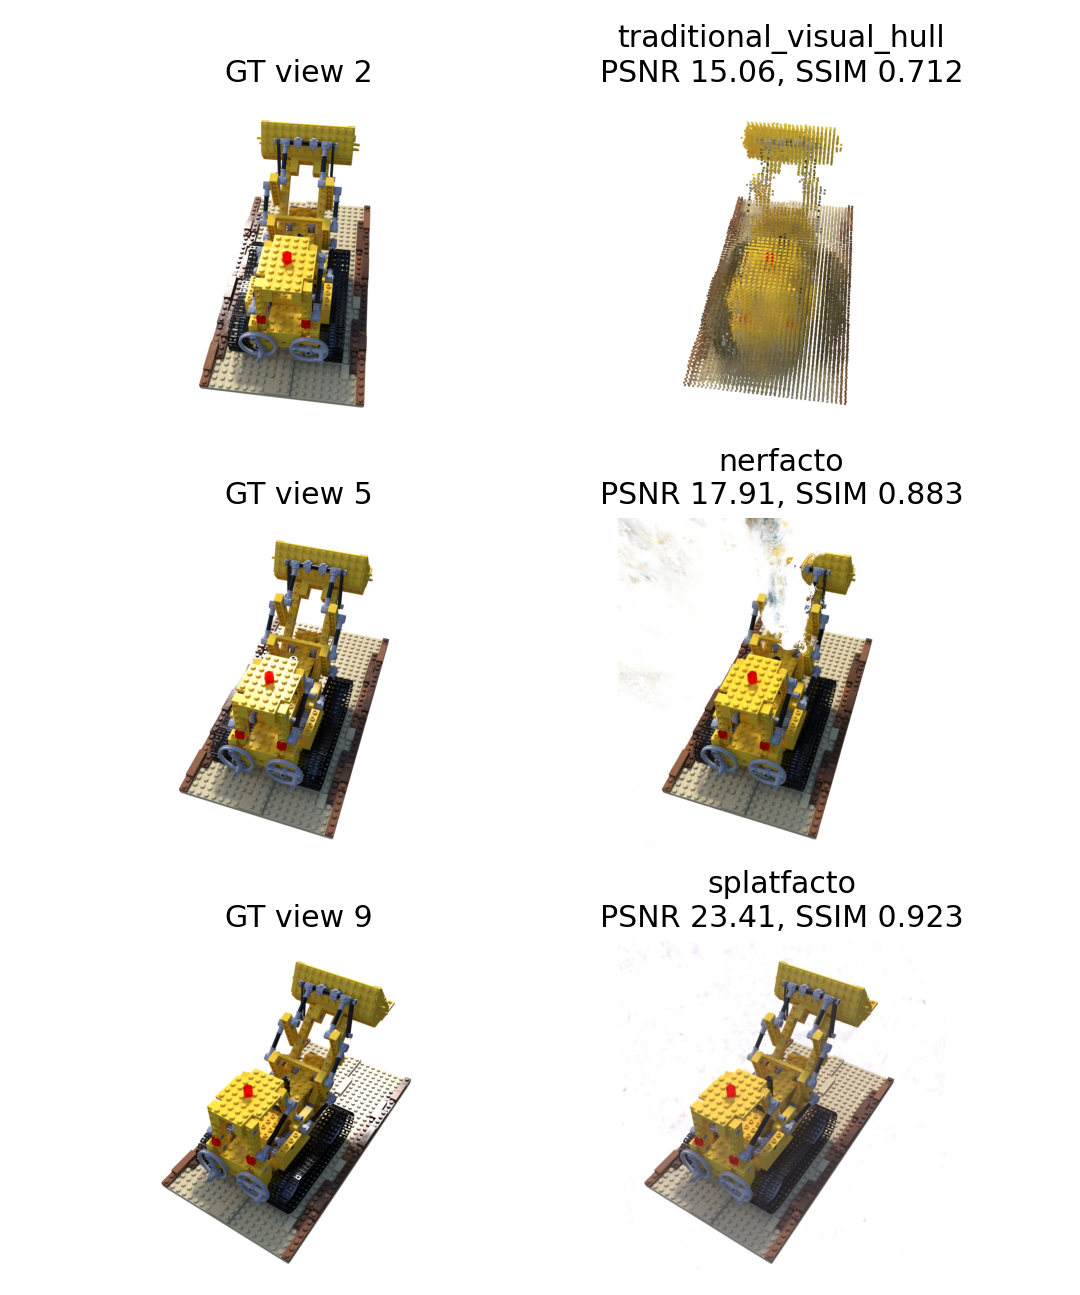
\includegraphics[width=0.75\textwidth]{images/experiments/lego_failure_cases.png}
\caption{三种方法在各自 PSNR 最差视角上的误差案例。Visual Hull 主要表现为轮廓外壳缺失与点状破碎，Nerfacto 主要表现为边缘软化和背景残留，Splatfacto 主要表现为局部颜色漂移或残余浮点。}
\label{fig:failure-cases}
\end{figure}

图 \ref{fig:comparison} 显示，Visual Hull 能够恢复 Lego 模型的大致轮廓，但点云条纹、孔洞和颜色混叠较明显，尤其在顶部细杆、车轮和底座边缘处容易破碎。其根本原因是 visual hull 只能恢复所有轮廓锥的交集，无法表达轮廓内部的凹陷、遮挡和视角相关外观。Nerfacto 能更完整地保持物体整体结构，但部分视角出现边缘软化，这与辐射场体渲染中的密度扩散和采样平均有关。Splatfacto 的边缘和高亮区域更锐利，但在最差视角中仍可能出现局部漂浮高斯或颜色偏移。图 \ref{fig:failure-cases} 说明，不同方法的失败机制并不相同：显式基线受几何外壳限制，NeRF 类方法受连续体场平滑与采样影响，3DGS 则受离散高斯的分布、尺度和排序影响。

\subsection{消融实验与待补实验}
当前实验已经完成三种流程在单一受控合成场景上的对比，但仍不足以支撑对复杂材质和真实场景的泛化结论。后续实验应至少补充三类内容：第一，在 \texttt{materials}、\texttt{drums}、\texttt{ficus} 等场景上重复相同评估，以验证高光、曲面、细结构和自遮挡下的稳定性（\texttt{TODO\_4}）；第二，加入真实采集场景或 Nerfstudio 官方真实场景数据，以验证相机噪声、背景干扰和真实光照变化的影响（\texttt{TODO\_3}）；第三，设计输入视角数量或训练迭代数消融，观察稀疏视角和优化步数对 PSNR、SSIM、LPIPS、失败视角和渲染时间的影响（\texttt{TODO\_6}）。这些补充实验完成后，才能将本文结论从单场景验证扩展到更一般的三维重建管线比较。

\section{结果讨论}
\subsection{结果质量}
在 Lego 场景上，神经渲染方法相对于传统显式基线具有明确的图像质量优势。Nerfacto 相比 Visual Hull 提高 5.51 dB PSNR，Splatfacto 相比 Visual Hull 提高 12.66 dB PSNR；SSIM 也从 0.701 分别提高到 0.873 和 0.955。这一结果说明，在训练视角覆盖充分且相机准确的条件下，图像监督下的连续或半显式表示比单纯依赖轮廓外壳更适合新视角合成。该结论目前只对受控合成场景成立；复杂材质和真实场景仍需 \texttt{TODO\_3} 与 \texttt{TODO\_4} 验证。

\subsection{控制性}
控制性并未随图像质量同步提高。Visual Hull 的中间结果是显式点云/体素，可进一步转为网格并进行几何检查；其缺点是几何不完整时图像质量直接下降。Nerfacto 把几何、颜色和可见性编码在连续辐射场中，难以直接编辑单个面片、UV 或材质节点。Splatfacto 的三维高斯比纯 MLP 场更局部、更可选择，但仍缺少稳定拓扑和物理材质分解。因此，神经渲染提升了从图像到新视角结果的自动化程度，却削弱了传统图形学中“几何、材质、光照分离编辑”的直接性。

\subsection{效率}
从理论上看，NeRF 类方法的渲染代价受 $HW N_s C_{\mathrm{MLP}}$ 控制，计算集中在沿射线采样和 MLP 查询；3DGS 将代价转移到高斯投影、tile 排序和 alpha 合成，更适合 GPU 并行渲染。实验中 Visual Hull 的构建时间约为 7.73 s，单测试视角点 splatting 平均约为 1.24 s；Nerfacto 和 Splatfacto 的真实单帧渲染时间尚未在统一环境中复测，因此以 \texttt{TODO\_2} 标记。现有结果可以支持“神经表示提高图像质量”的判断，但不能据此声称完整流程耗时已经优于传统方法。

\subsection{局限与失败机理}
神经渲染的失败并非随机现象，而与表示方式直接相关。NeRF 类方法在稀疏视角或遮挡边界处容易出现模糊，是因为体密度和颜色需要从有限图像监督中解释连续空间，多个可能表面会被平均到同一射线积分中。3DGS 在局部区域出现漂浮点或颜色漂移，则与离散高斯的尺度、透明度、深度排序和视角覆盖不足有关。传统显式流程的失败更直接，主要来自特征匹配、轮廓外壳或网格重建本身不完整。由此可见，神经渲染并不是消除重建困难，而是把显式几何修复问题转化为可微表示优化问题，并引入新的稳定性和可解释性代价。

\section{结论与展望}
本文围绕三维场景重建与新视角渲染任务，比较了传统显式重建流程、NeRF 类神经辐射场流程和 3DGS 类高效神经渲染流程。理论分析表明，三类方法的核心差异在于场景表示和渲染代价：传统流程依赖可编辑网格与材质，NeRF 依赖逐射线体渲染和 MLP 查询，3DGS 则通过半显式高斯和 splatting 将渲染推向更接近光栅化的并行过程。Lego 场景实验显示，Nerfacto 和 Splatfacto 在 PSNR 与 SSIM 上均优于 Visual Hull，其中 Splatfacto 获得最高平均质量，但其跨视角方差和局部失败案例仍提示稳定性问题。

本文的主要局限在于实验场景数量不足，LPIPS、统一渲染时间、真实场景验证和消融实验尚未全部完成。后续工作应补充多场景与真实场景数据，统一报告 PSNR、SSIM、LPIPS、渲染时间、显存占用、最差视角和失败案例，并进一步比较 SuGaR、GaussianShader、2DGS 等面向几何提取与材质建模的 3DGS 扩展方法。只有在质量、效率、控制性和失败机制四个维度上同时给出证据，才能更完整地评价神经渲染相对于传统图形学流程的优势和代价。
\begin{thebibliography}{99}
\bibitem{tewari2020state} A. Tewari, O. Fried, J. Thies, V. Sitzmann, S. Lombardi, K. Sunkavalli, R. Martin-Brualla, T. Simon, J. Saragih, M. Nie{\ss}ner, et al. State of the Art on Neural Rendering. Computer Graphics Forum, 39(2):701--727, 2020.
\bibitem{xie2022neuralfields} Y. Xie, T. Takikawa, S. Saito, O. Litany, S. Yan, N. Khan, F. Tombari, J. Tompkin, V. Sitzmann, and S. Sridhar. Neural Fields in Visual Computing and Beyond. Computer Graphics Forum, 41(2):641--676, 2022.
\bibitem{mildenhall2020nerf} B. Mildenhall, P. P. Srinivasan, M. Tancik, J. T. Barron, R. Ramamoorthi, and R. Ng. NeRF: Representing Scenes as Neural Radiance Fields for View Synthesis. In Proceedings of the European Conference on Computer Vision, pp. 405--421, 2020.
\bibitem{muller2022instant} T. M{\"u}ller, A. Evans, C. Schied, and A. Keller. Instant Neural Graphics Primitives with a Multiresolution Hash Encoding. ACM Transactions on Graphics, 41(4):102:1--102:15, 2022.
\bibitem{yu2022plenoxels} A. Yu, S. Fridovich-Keil, M. Tancik, Q. Chen, B. Recht, and A. Kanazawa. Plenoxels: Radiance Fields without Neural Networks. In Proceedings of the IEEE/CVF Conference on Computer Vision and Pattern Recognition, pp. 5501--5510, 2022.
\bibitem{chen2022tensorf} A. Chen, Z. Xu, A. Geiger, J. Yu, and H. Su. TensoRF: Tensorial Radiance Fields. In Proceedings of the European Conference on Computer Vision, pp. 333--350, 2022.
\bibitem{barron2021mipnerf} J. T. Barron, B. Mildenhall, M. Tancik, P. Hedman, R. Martin-Brualla, and P. P. Srinivasan. Mip-NeRF: A Multiscale Representation for Anti-Aliasing Neural Radiance Fields. In Proceedings of the IEEE/CVF International Conference on Computer Vision, pp. 5855--5864, 2021.
\bibitem{kerbl2023gaussians} B. Kerbl, G. Kopanas, T. Leimk{\"u}hler, and G. Drettakis. 3D Gaussian Splatting for Real-Time Radiance Field Rendering. ACM Transactions on Graphics, 42(4):139:1--139:14, 2023.
\bibitem{schonberger2016sfm} J. L. Sch{\"o}nberger and J.-M. Frahm. Structure-from-Motion Revisited. In Proceedings of the IEEE Conference on Computer Vision and Pattern Recognition, pp. 4104--4113, 2016.
\bibitem{schonberger2016mvs} J. L. Sch{\"o}nberger, E. Zheng, M. Pollefeys, and J.-M. Frahm. Pixelwise View Selection for Unstructured Multi-View Stereo. In Proceedings of the European Conference on Computer Vision, pp. 501--518, 2016.
\bibitem{sitzmann2019srn} V. Sitzmann, M. Zollh{\"o}fer, and G. Wetzstein. Scene Representation Networks: Continuous 3D-Structure-Aware Neural Scene Representations. In Advances in Neural Information Processing Systems, 2019.
\bibitem{park2019deepsdf} J. J. Park, P. Florence, J. Straub, R. Newcombe, and S. Lovegrove. DeepSDF: Learning Continuous Signed Distance Functions for Shape Representation. In Proceedings of the IEEE/CVF Conference on Computer Vision and Pattern Recognition, pp. 165--174, 2019.
\bibitem{tancik2020fourier} M. Tancik, P. P. Srinivasan, B. Mildenhall, S. Fridovich-Keil, N. Raghavan, U. Singhal, R. Ramamoorthi, J. T. Barron, and R. Ng. Fourier Features Let Networks Learn High Frequency Functions in Low Dimensional Domains. In Advances in Neural Information Processing Systems, 2020.
\bibitem{barron2022mipnerf360} J. T. Barron, B. Mildenhall, D. Verbin, P. P. Srinivasan, and P. Hedman. Mip-NeRF 360: Unbounded Anti-Aliased Neural Radiance Fields. In Proceedings of the IEEE/CVF Conference on Computer Vision and Pattern Recognition, pp. 5470--5479, 2022.
\bibitem{barron2023zipnerf} J. T. Barron, B. Mildenhall, D. Verbin, P. P. Srinivasan, and P. Hedman. Zip-NeRF: Anti-Aliased Grid-Based Neural Radiance Fields. In Proceedings of the IEEE/CVF International Conference on Computer Vision, pp. 19697--19705, 2023.
\bibitem{yu2021plenoctrees} A. Yu, R. Li, M. Tancik, H. Li, R. Ng, and A. Kanazawa. PlenOctrees for Real-Time Rendering of Neural Radiance Fields. In Proceedings of the IEEE/CVF International Conference on Computer Vision, pp. 5752--5761, 2021.
\bibitem{hedman2021snerg} P. Hedman, P. P. Srinivasan, B. Mildenhall, J. T. Barron, and P. Debevec. Baking Neural Radiance Fields for Real-Time View Synthesis. In Proceedings of the IEEE/CVF International Conference on Computer Vision, pp. 5875--5884, 2021.
\bibitem{jiang2023gaussianshader} Y. Jiang, J. Tu, Y. Liu, X. Gao, X. Long, W. Wang, and Y. Ma. GaussianShader: 3D Gaussian Splatting with Shading Functions for Reflective Surfaces. arXiv preprint arXiv:2311.17977, 2023.
\bibitem{wang2023gaussianeditor} J. Wang, J. Fang, X. Zhang, L. Xie, and Q. Tian. GaussianEditor: Editing 3D Gaussians Delicately with Text Instructions. arXiv preprint arXiv:2311.16037, 2023.
\bibitem{guedon2023sugar} A. Gu{\'e}don and V. Lepetit. SuGaR: Surface-Aligned Gaussian Splatting for Efficient 3D Mesh Reconstruction and High-Quality Mesh Rendering. arXiv preprint arXiv:2311.12775, 2023.
\bibitem{huang2024twodgs} B. Huang, Z. Yu, A. Chen, A. Geiger, and S. Gao. 2D Gaussian Splatting for Geometrically Accurate Radiance Fields. arXiv preprint arXiv:2403.17888, 2024.
\bibitem{wang2021neus} P. Wang, L. Liu, Y. Liu, C. Theobalt, T. Komura, and W. Wang. NeuS: Learning Neural Implicit Surfaces by Volume Rendering for Multi-View Reconstruction. In Advances in Neural Information Processing Systems, 2021.
\bibitem{yariv2021volsdf} L. Yariv, J. Gu, Y. Kasten, and Y. Lipman. Volume Rendering of Neural Implicit Surfaces. In Advances in Neural Information Processing Systems, 2021.
\bibitem{lin2021barf} C.-H. Lin, W.-C. Ma, A. Torralba, and S. Lucey. BARF: Bundle-Adjusting Neural Radiance Fields. In Proceedings of the IEEE/CVF International Conference on Computer Vision, pp. 5741--5751, 2021.
\bibitem{martinbrualla2021nerfw} R. Martin-Brualla, N. Radwan, M. S. M. Sajjadi, J. T. Barron, A. Dosovitskiy, and D. Duckworth. NeRF in the Wild: Neural Radiance Fields for Unconstrained Photo Collections. In Proceedings of the IEEE/CVF Conference on Computer Vision and Pattern Recognition, pp. 7210--7219, 2021.
\bibitem{niemeyer2022regnerf} M. Niemeyer, J. T. Barron, B. Mildenhall, M. Nie{\ss}ner, and A. Geiger. RegNeRF: Regularizing Neural Radiance Fields for View Synthesis from Sparse Inputs. In Proceedings of the IEEE/CVF Conference on Computer Vision and Pattern Recognition, pp. 5480--5490, 2022.
\end{thebibliography}

\end{document}
